\documentclass[tikz,border=8pt]{standalone}
\begin{document}
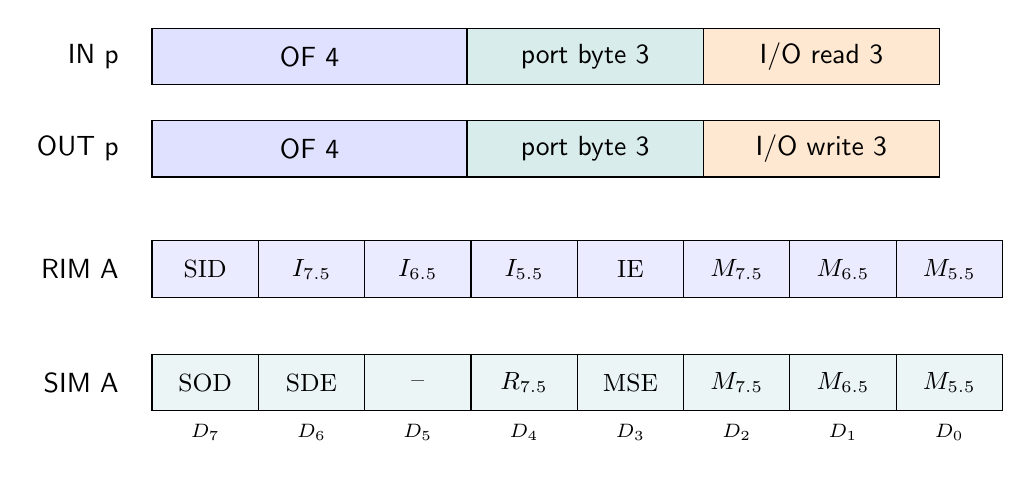
\begin{tikzpicture}[font=\sffamily,x=1cm,y=.9cm]
\node[anchor=east] at (-.3,5.8){IN p};\draw[fill=blue!12] (0,5.4) rectangle (4,6.2);\node at (2,5.8){OF 4};\draw[fill=teal!15] (4,5.4) rectangle (7,6.2);\node at (5.5,5.8){port byte 3};\draw[fill=orange!18] (7,5.4) rectangle (10,6.2);\node at (8.5,5.8){I/O read 3};
\node[anchor=east] at (-.3,4.5){OUT p};\draw[fill=blue!12] (0,4.1) rectangle (4,4.9);\node at (2,4.5){OF 4};\draw[fill=teal!15] (4,4.1) rectangle (7,4.9);\node at (5.5,4.5){port byte 3};\draw[fill=orange!18] (7,4.1) rectangle (10,4.9);\node at (8.5,4.5){I/O write 3};
\node[anchor=east] at (-.3,2.8){RIM A};
\foreach \x/\v in {0/SID,1/$I_{7.5}$,2/$I_{6.5}$,3/$I_{5.5}$,4/IE,5/$M_{7.5}$,6/$M_{6.5}$,7/$M_{5.5}$}{\draw[fill=blue!8] (\x*1.35,2.4) rectangle ++(1.35,.8);\node[font=\small] at (\x*1.35+.675,2.8){\v};}
\node[anchor=east] at (-.3,1.2){SIM A};
\foreach \x/\v in {0/SOD,1/SDE,2/--,3/$R_{7.5}$,4/MSE,5/$M_{7.5}$,6/$M_{6.5}$,7/$M_{5.5}$}{\draw[fill=teal!8] (\x*1.35,.8) rectangle ++(1.35,.8);\node[font=\small] at (\x*1.35+.675,1.2){\v};}
\foreach \x/\v in {0/$D_7$,1/$D_6$,2/$D_5$,3/$D_4$,4/$D_3$,5/$D_2$,6/$D_1$,7/$D_0$}{\node[font=\scriptsize] at (\x*1.35+.675,.5){\v};}
\end{tikzpicture}
\end{document}
